\chapter{Zusammenarbeit und soziale Funktion}
\label{ch:zusammenarbeit}

\section{Freunde}% Screenshot von beiden Seiten (Menü und nutzerseite)
\label{sec:freunde}
PUMA bietet den Nutzern die Möglichkeit, andere Nutzer als Freunde zu kennzeichnen. Freundschaften\index{Freunde} ermöglichen das Teilen von Publikationen und Lesezeichen. Dazu in der Sichtbarkeitseinstellung eines Eintrags \enquote{andere} und dann \enquote{friends} auswählen, dann können zusätzlich \enquote{Freunde} diesen Eintrag sehen. Auf die gleiche Weise können Freunde Einträge sichtbar machen. Einen Überblick über diese Einträge erhält man über den Menüeintrag \enquote{meinPUMA} (\autoref{subsec:meinPuma}) unter \enquote{Einträge von Freunden} bzw. \enquote{Einträge für Freunde}.\newline

\subsection{Freund hinzufügen}
\label{subsec:freundHinzu}

Entweder auf den Benutzernamen unter einem Eintrag klicken oder im Suchfeld auf Benutzer einschränken oder in der allgemeinen Suche user:Benutzername eingeben (\autoref{sec:suche}).Eine Seite des Nutzers wird angezeigt, auf der alle öffentlichen Einträge zu sehen sind. In der rechten Menüleiste wird der Name eingeblendet darunter besteht die Möglichkeit diesen Nutzer über als Freund hinzuzufügen.
    
		
		%\begin{figure}[h!]
 %\centering
 %\fbox{\includegraphics[width=5cm]{Bilder/Kapitel8/Benutzername_in_Eintrag}}
 %\caption{Benutzername anklicken}
 %\label{fig:benutzerAnklicken}
%\end{figure}

		\begin{figure}[h!]
 \centering
 \fbox{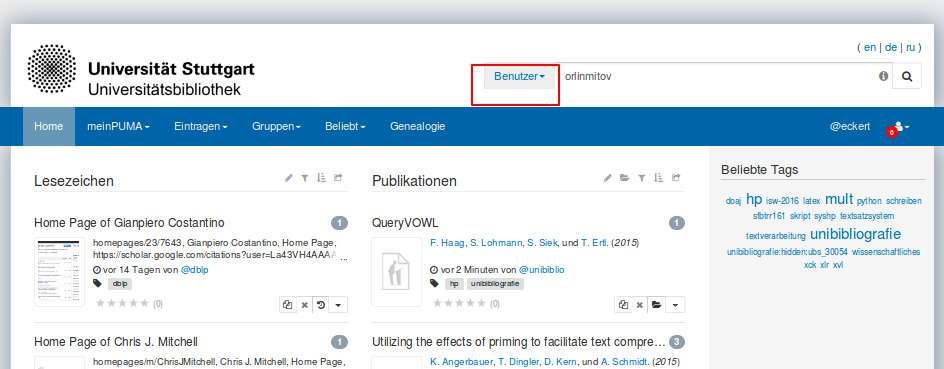
\includegraphics[width=11cm]{Bilder/Kapitel8/Benutzer_suchen}}
 \caption{Benutzer suchen}
 \label{fig:benutzerSuchen}
\end{figure}

\begin{figure}[h!]
 \centering
 \fbox{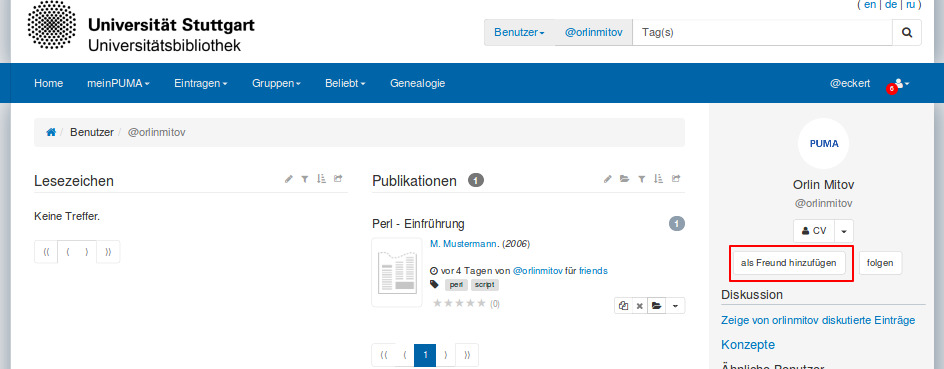
\includegraphics[width=11cm]{Bilder/Kapitel8/Nutzerseite}}
 \caption{Die Nutzerseite}
 \label{fig:nutzerseite}
\end{figure}

\subsection{Freundesübersicht}
\label{subsec:freundesuebersicht}
Die Freundesübersicht bietet einen Überblick über Freunde in PUMA. Zu der Übersicht gelangt man über das Dropdown-Menü des Personensymbols. Unter dem Reiter \enquote{Freunde} erhält man einen Überblick über Freunde und kann sehen, welche Nutzer einen als Freund angegeben hat. Am Ende der Seite sind alle Publikationen aufgelistet, die mit Freunden geteilt wurden oder Freunden geteilt haben.\newline

\begin{figure}[h!]
 \centering
 \fbox{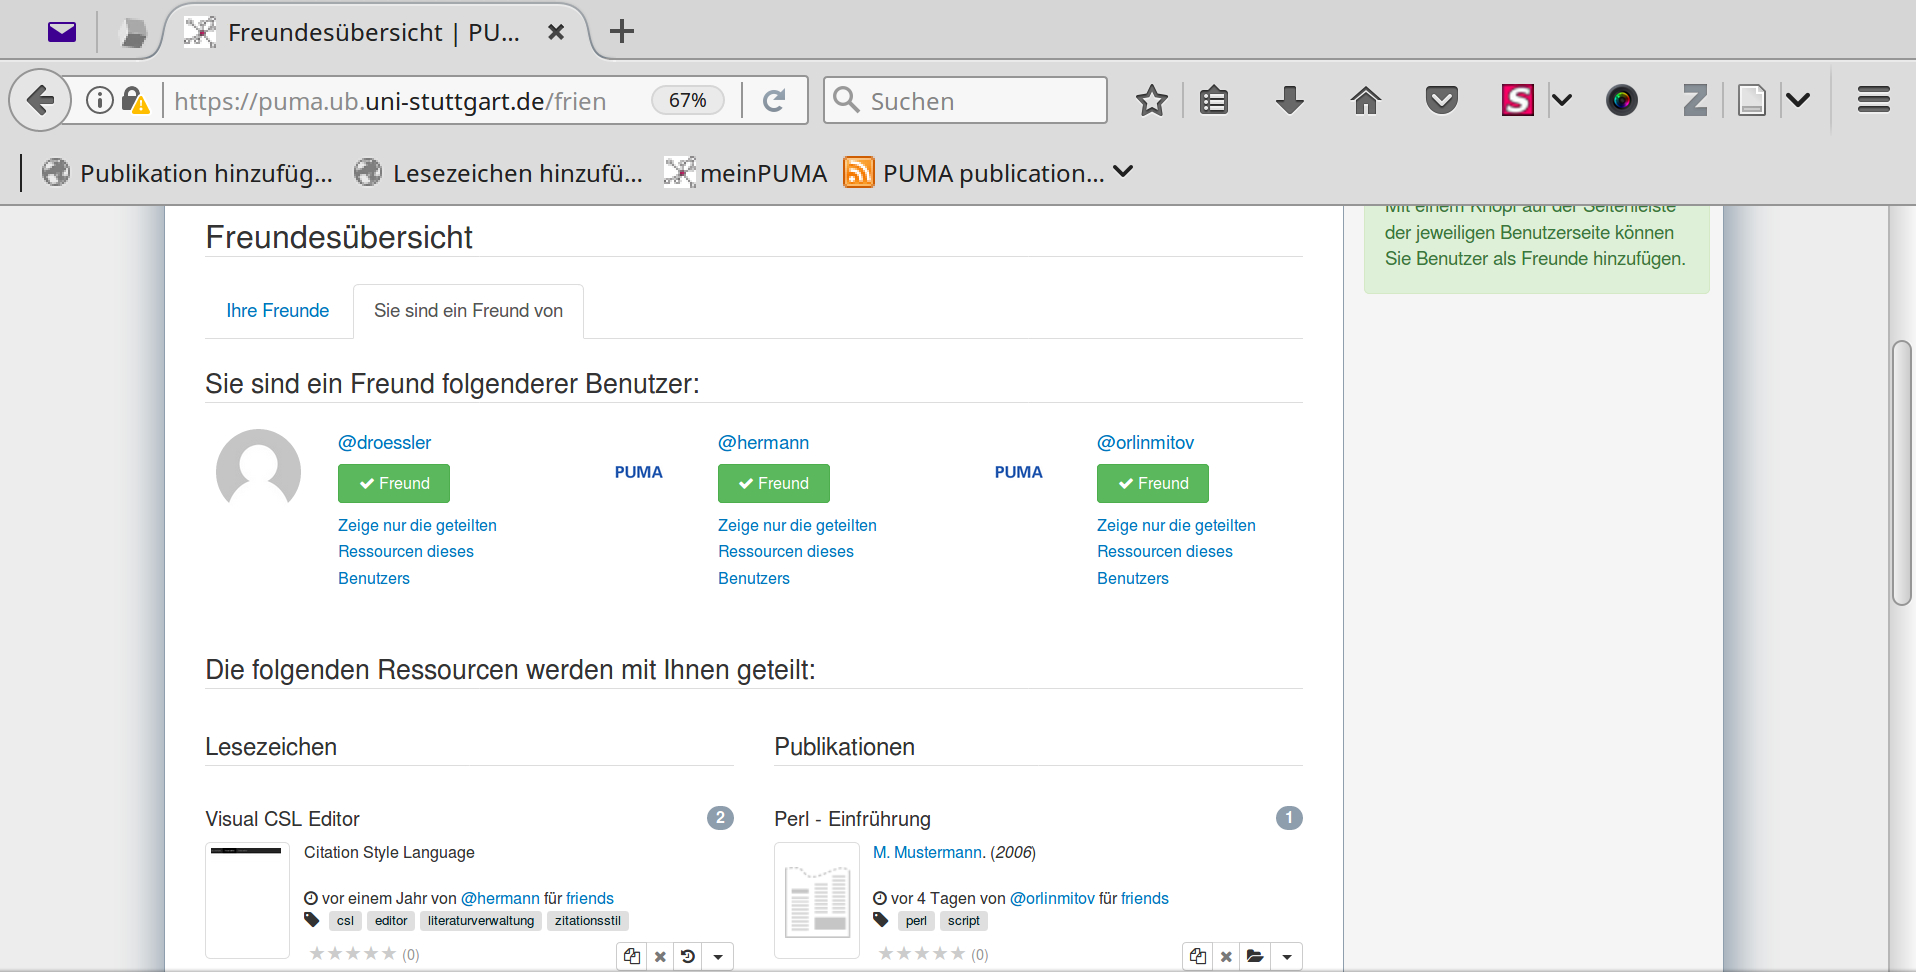
\includegraphics[width=11cm]{Bilder/Kapitel8/Freundesuebersicht}}
 \caption{Freundesübersicht}
 \label{fig:freundesuebersicht}
\end{figure}

Es besteht jederzeit die Möglichkeit, Freunde wieder zu entfernen. Hierfür mit der Maus auf den jeweiligen grünen Kasten \enquote{Freund} des Freundes, der entfernt werden soll klicken.

\section{Gruppen}
\label{sec:gruppen}
Gruppen\index{Gruppen} vereinfachen die Zusammenarbeit auf Puma. Sie ermöglichen eine gemeinsame Literaturrecherche und erleichtern so die Umsetzung von gemeinsamen Projekten. Gleichzeitig kann innerhalb einer Institution oder Arbeitsgruppe der Austausch über neue, interessante, fremde oder eigene Artikel mit Hilfe von PUMA erfolgen und somit die Kommunikation vereinfacht werden.

\subsection{Gruppen \index{Gruppen!beitreten}suchen und beitreten}
\label{subsec:gruppenSuchenBeitreten}

\begin{figure}[h!]
 \centering
 \fbox{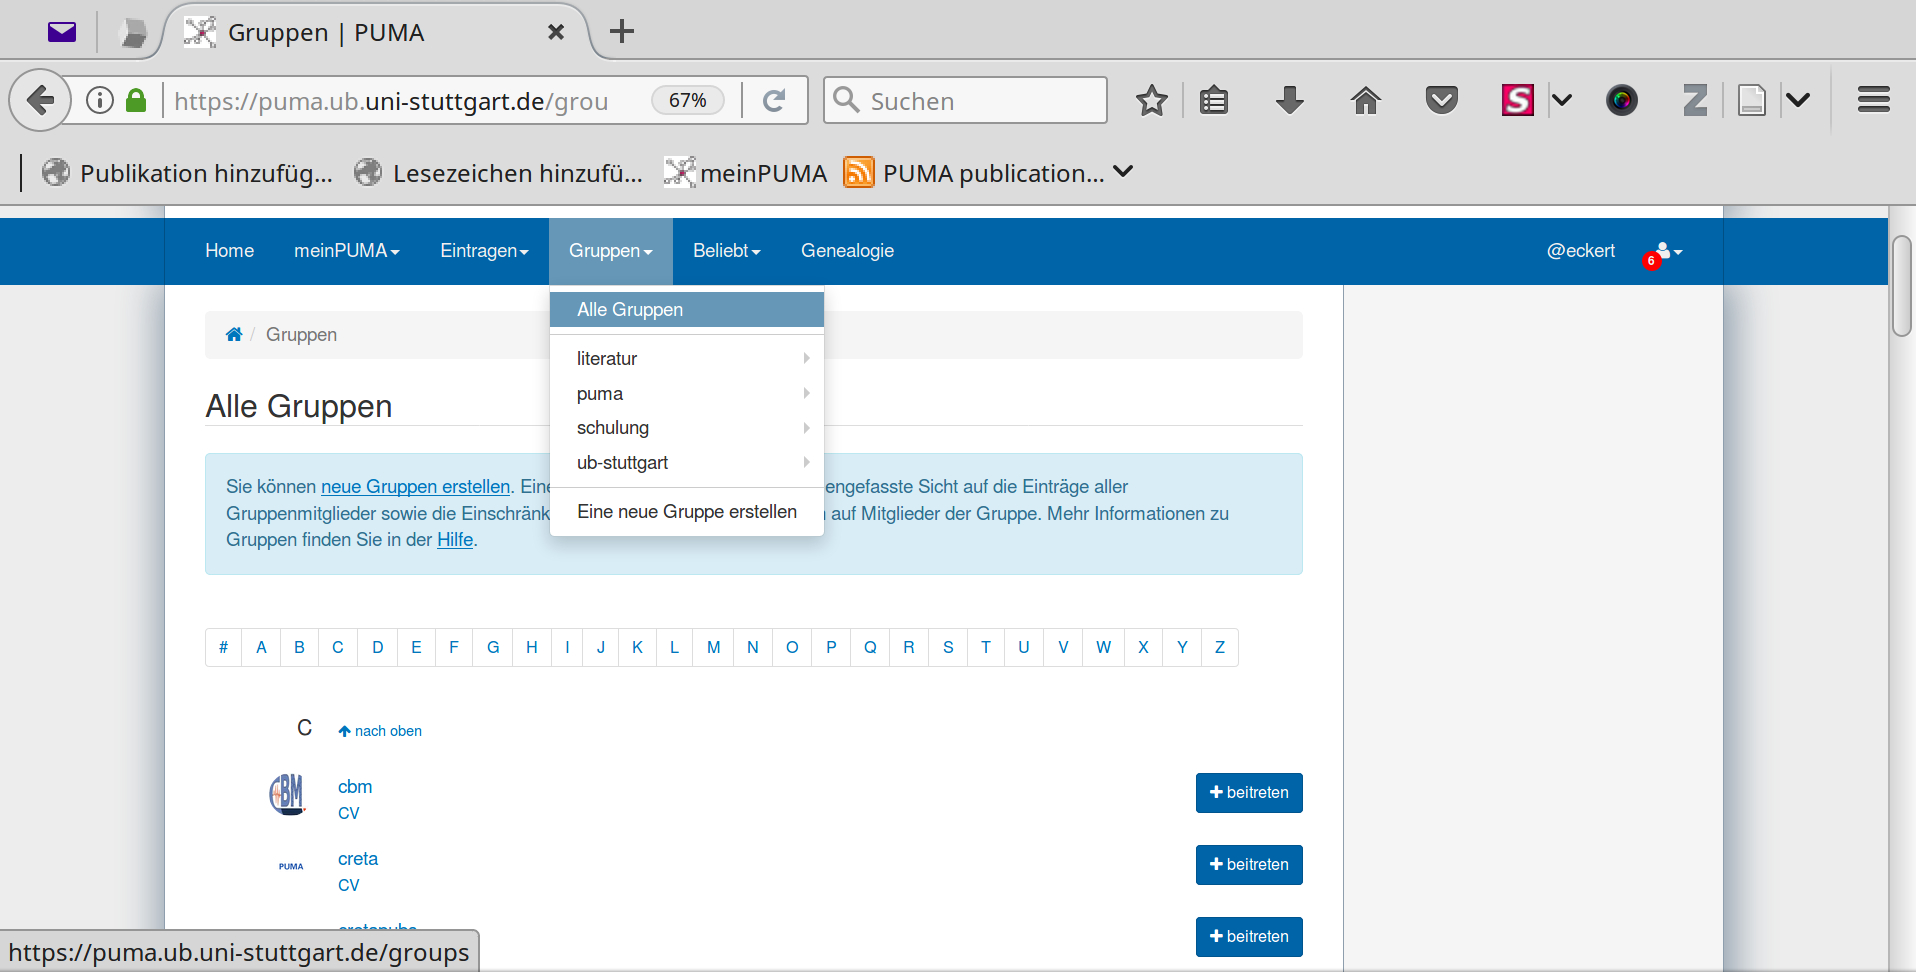
\includegraphics[width=11cm]{Bilder/Kapitel8/Gruppen-Uebersichtsseite}}
 \caption{Allgemeine Liste}
 \label{fig:allgemeineListe}
\end{figure}
\begin{enumerate}

Im Hauptmenü \enquote{Gruppen} im . Ein Dropdown-Menü öffnet sich.
    \item Klicken Sie im Dropdown-Menü auf \enquote{Alle Gruppen}.
    \item Es öffnet sich eine Übersicht über alle Gruppen bei PUMA in alphabetischer Reihenfolge. Rechts neben dem jeweiligen Gruppennamen befindet sich ein Button, um der Gruppe beizutreten. Klicken Sie auf den Beitreten-Button der gewünschten Gruppe.
\begin{figure}[h!]
 \centering
 \fbox{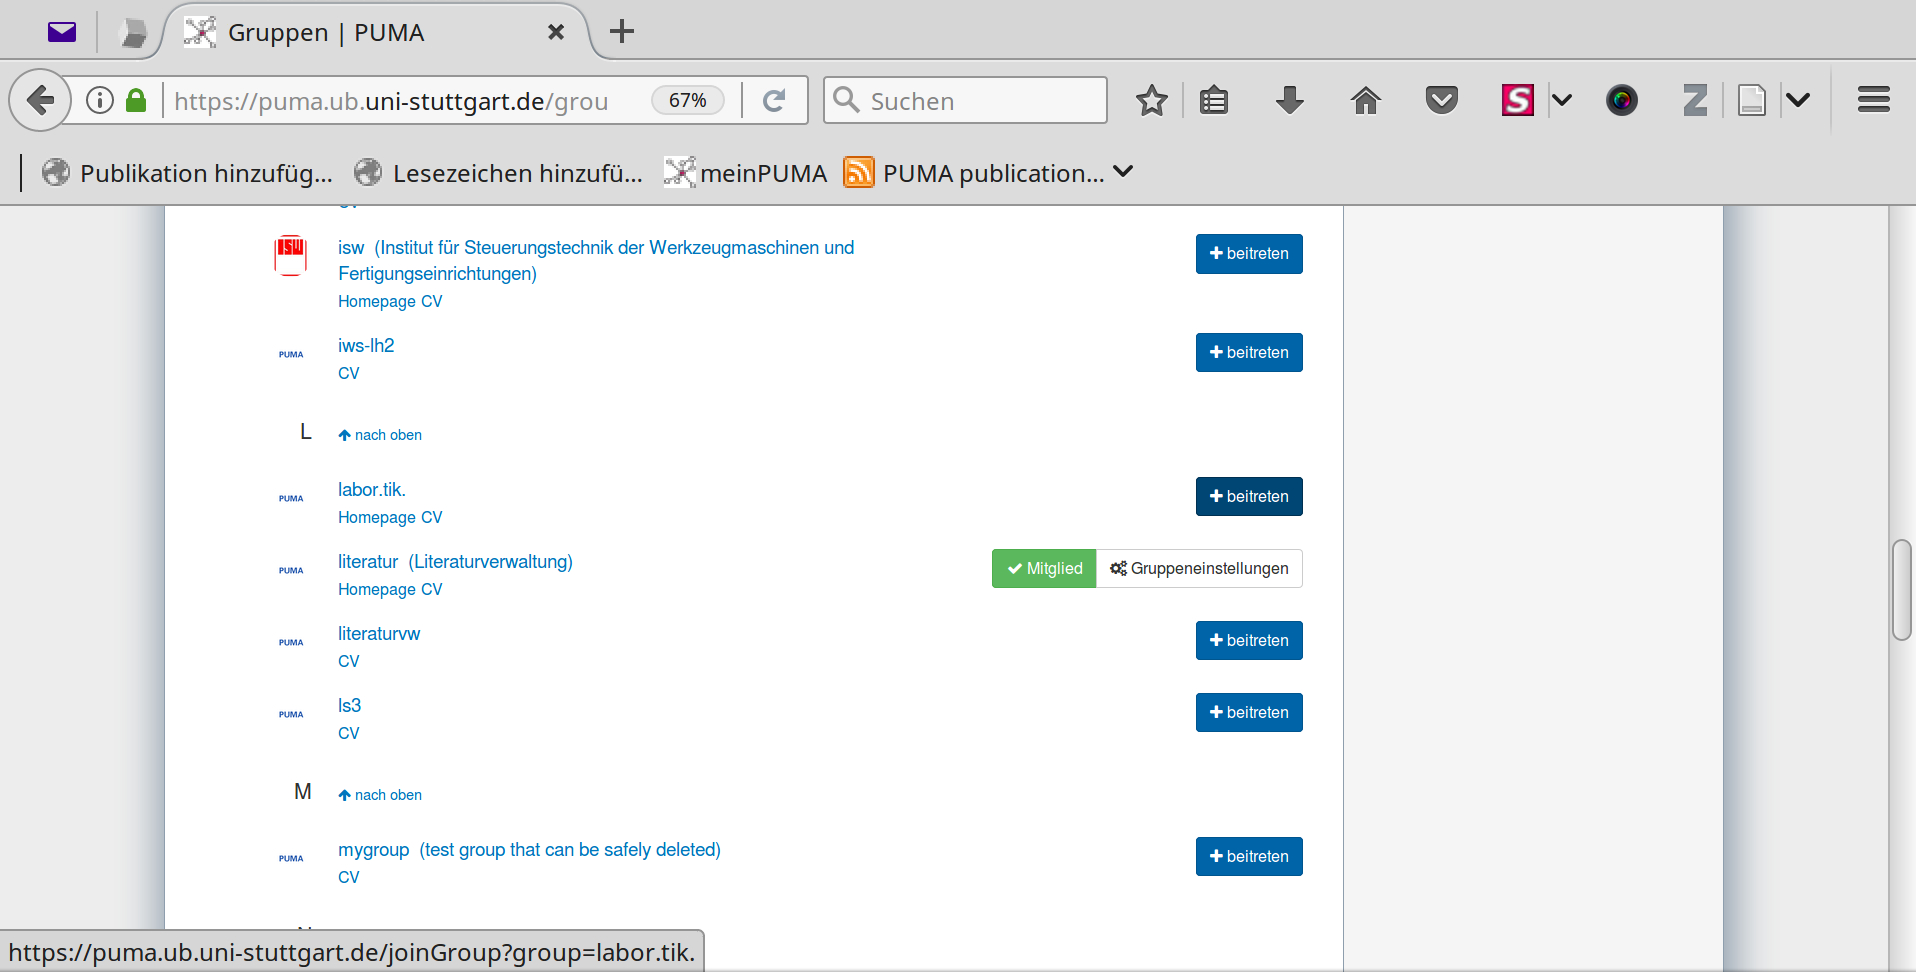
\includegraphics[width=11cm]{Bilder/Kapitel8/Beitreten_einer_Gruppe}}
 \caption{Beitreten einer Gruppe}
 \label{fig:gruppeBeitreten}
\end{figure}
    \item Eine neue Seite erscheint. Geben Sie in das Feld \enquote{Begründung} ein, warum Sie der Gruppe beitreten möchten.
    \item Geben Sie den angezeigten Captcha-Text in das vorgegebene Feld ein. Damit soll verhindert werden, dass Programme automatisiert Gruppen beitreten. 
    \item Klicken Sie anschließend auf \enquote{Anfrage absenden}.
    \item Der Gruppen-Administrator erhält eine E-Mail-Benachrichtigung, dass Sie in die Gruppe eintreten wollen. Allein der Administrator entscheidet über die Aufnahme, weswegen ein plausibler Begründungstext sinnvoll ist.
\end{enumerate}
In der E-Mail, die alle Administratoren erhalten, befindet sich ein Link (erster Link in der E-Mail). Durch das Anklicken des Links öffnet sich die Einstellungsseite der Gruppe. Der Administrator kann nun den Nutzer aufnehmen oder dessen Beitrittsanfrage ablehnen.
\subsection{Gruppen erstellen\index{Gruppen!erstellen}}
\label{subsec:gruppenErstellen}
\begin{enumerate}
    \item Klicken Sie im Hauptmenü auf \enquote{Gruppen}. Ein Dropdown-Menü öffnet sich.
    \item Klicken Sie im Dropdown-Menü auf \enquote{Eine neue Gruppe erstellen}.
\begin{figure}[h!]
 \centering
 \fbox{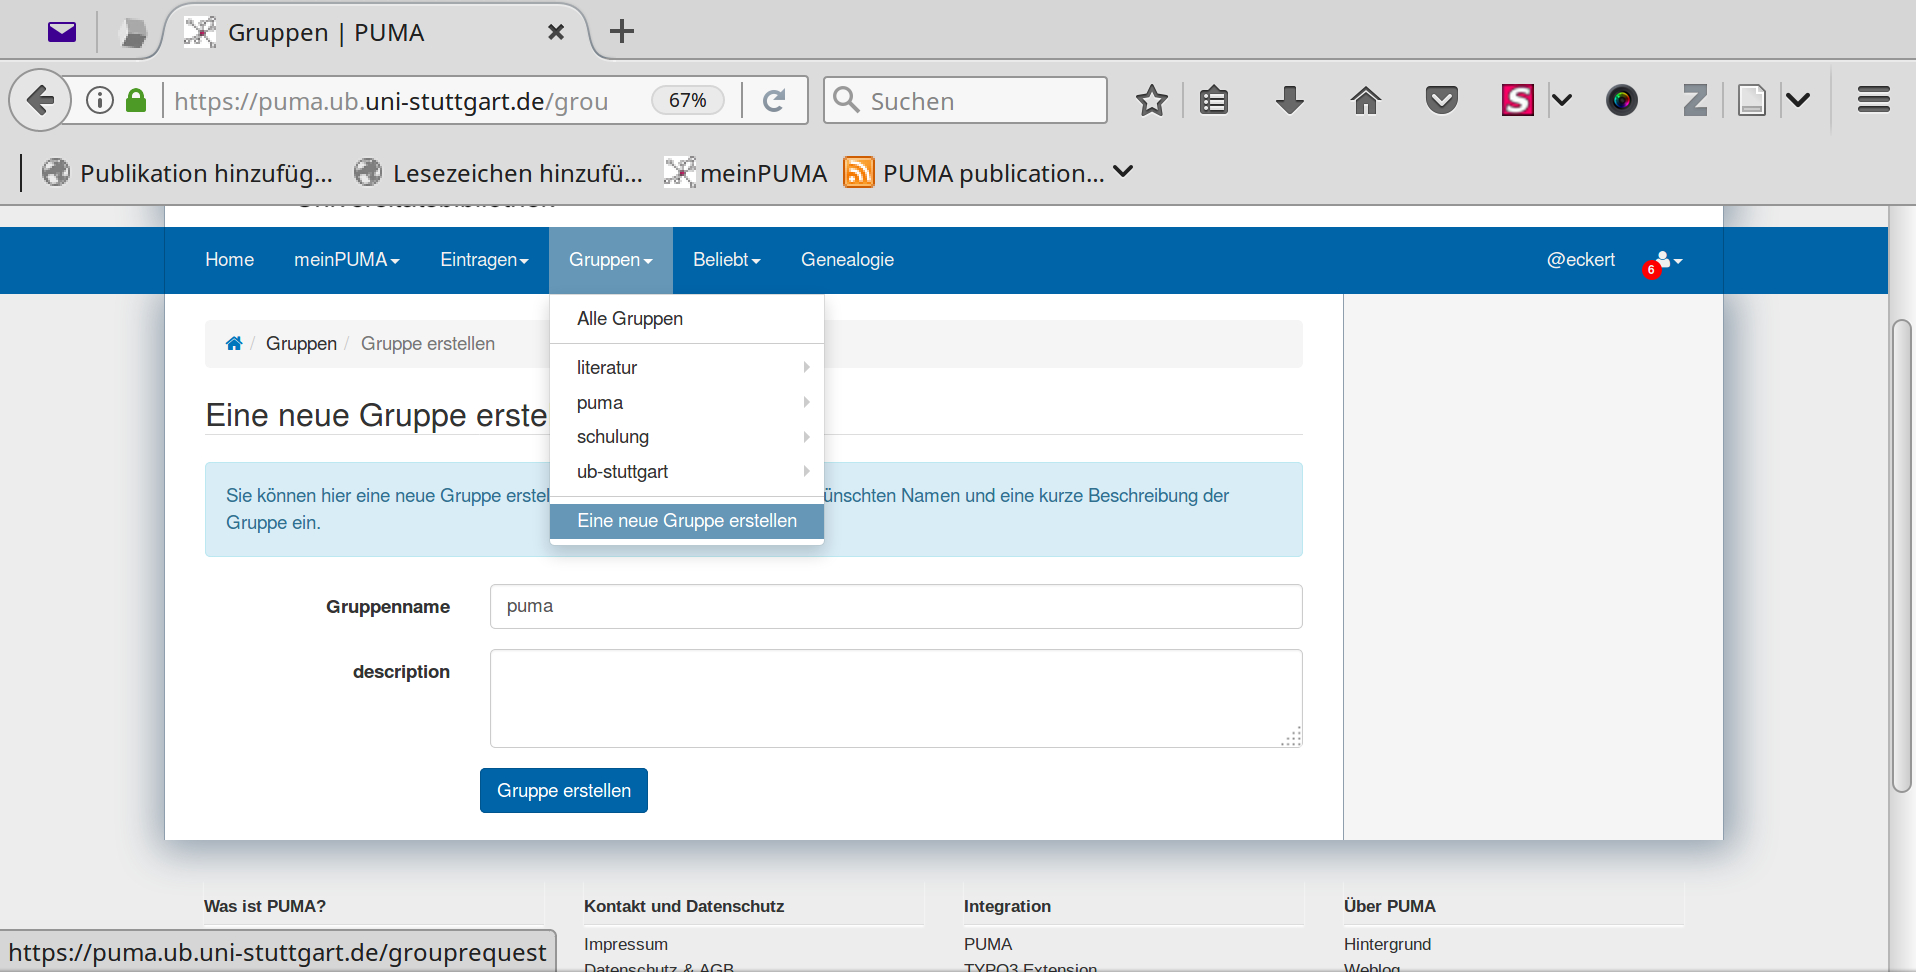
\includegraphics[width=11cm]{Bilder/Kapitel8/Neue_Gruppe_erstellen}}
 \caption{Erstellung einer neuen Gruppe}
 \label{fig:erstellungNeueGruppe}
\end{figure}
    \item Geben Sie einen Gruppennamen und eine Beschreibung der Gruppe an. 
    \item Klicken Sie anschließend auf \enquote{Gruppe erstellen}. 
\end{enumerate}
Ab sofort können Sie die Vorteile der gemeinsamen Literaturrecherche von PUMA nutzen und Publikationen für spezielle Gruppen sichtbar machen. Dies legen Sie beim Eintragen einer neuen Publikation oder eines neuen Lesezeichens fest, indem Sie bei der Sichtbarkeit\index{Sichtbarkeit} unter dem Punkt \textit{andere} die spezielle Gruppe auswählen. Wenn Sie diese Publikation nun speichern, sehen diese automatisch alle Gruppenmitglieder.
\subsection{Die Gruppenseite}
\label{subsec:gruppenseite}
Um zur Gruppenseite\index{Gruppen} zu gelangen, klicken Sie im Dropdown-Menü vom Reiter  \enquote{Gruppen} auf den entsprechenden Namen der Gruppe. Sie gelangen zur Gruppenseite, auf der Sie einen Überblick über alle Lesezeichen und Publikationen erhalten.%Screenshot
\newline\newline
Funktionen auf der Gruppenseite:
\begin{figure}[h!]
 \centering
 \fbox{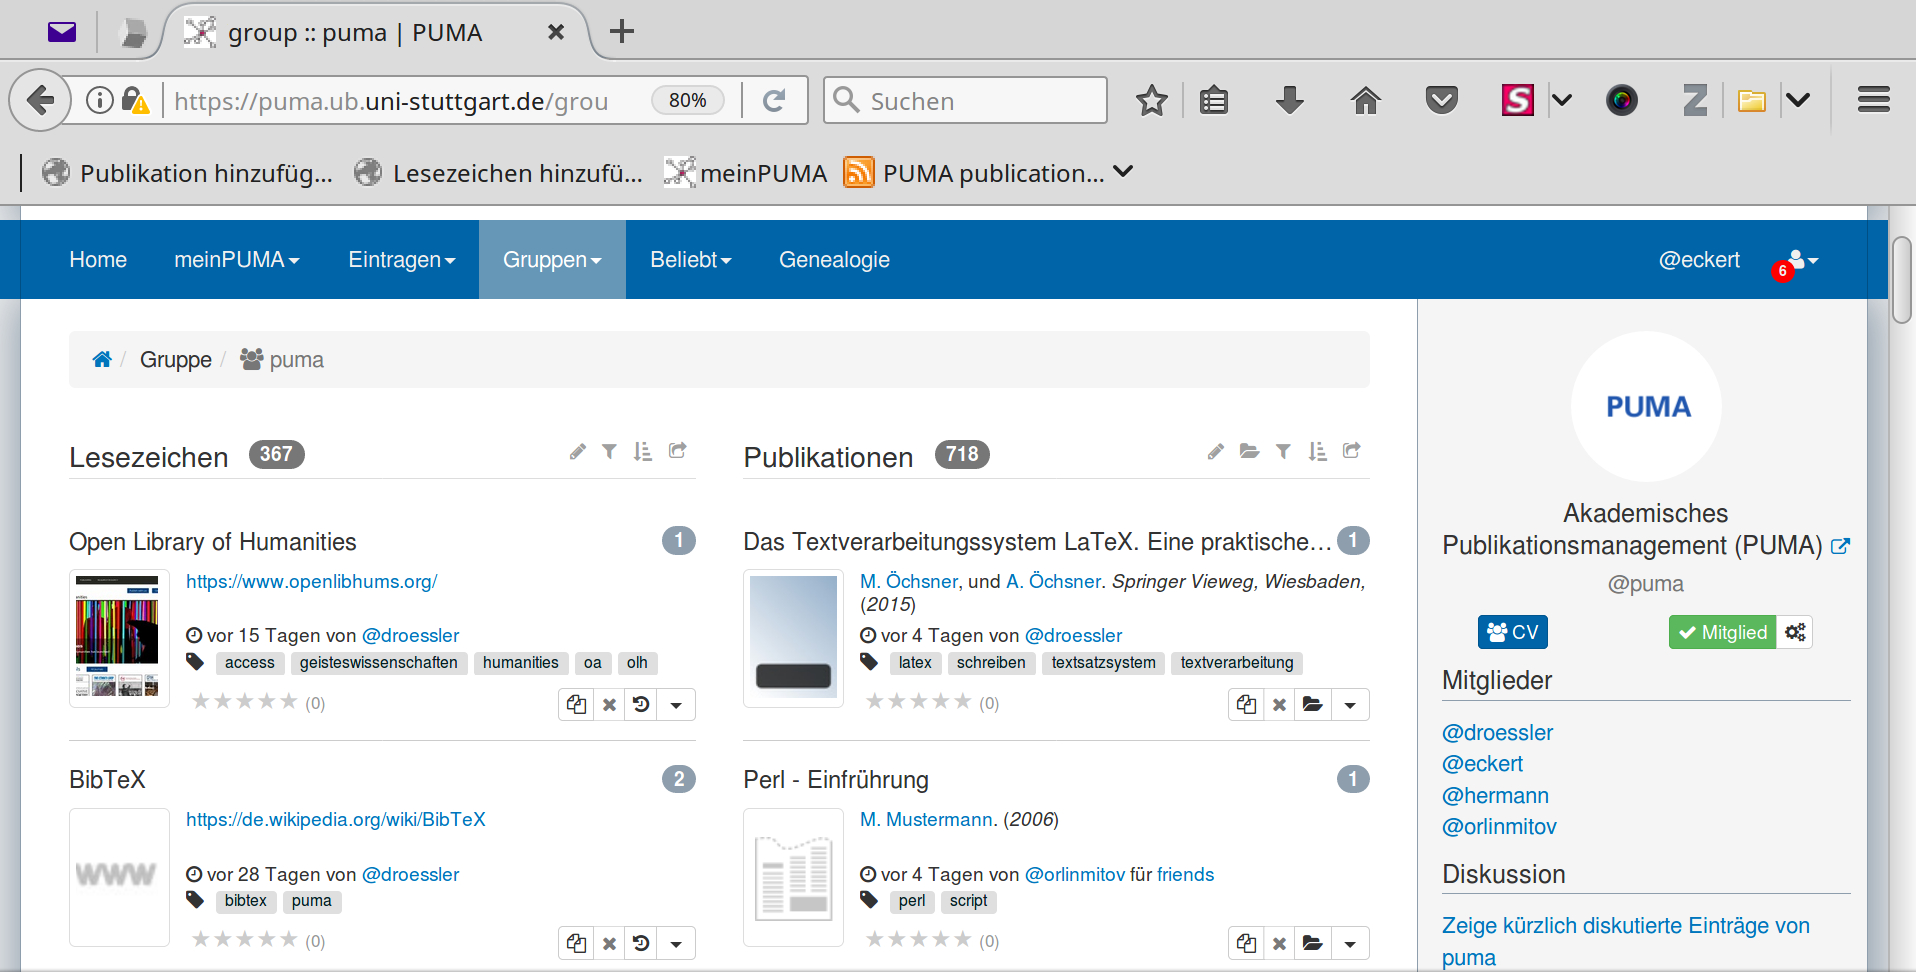
\includegraphics[width=11cm]{Bilder/Kapitel8/Gruppenseite}}
 \caption{Die Gruppenseite}
 \label{fig:gruppenseite}
\end{figure}
\begin{description}
\item [CV/Lebenslauf der Gruppe] \hfill \\
Durch Klicken auf den CV-Button auf der rechten Seite erhalten Sie alle wichtigen Informationen zu der Gruppe.
\item [Mitglieder-Liste] \hfill \\
Unterhalb des Gruppenbildes befindet sich die Liste aller Mitglieder. 
\item [Diskussionen] Um sich einen Überblick über die diskutierten Einträge zu verschaffen, klicken Sie unter dem Abschnitt Diskussion auf der rechten Seite auf \enquote{Zeige kürzlich diskutierte Einträge von PUMA}. 
\end{description}
 
\subsection{Rollen in einer Gruppe}
\label{subsec:RollenInGruppe}
In einer Gruppe können die unterschiedlichsten Rollen und Aufgaben übernommen werden. In PUMA gibt es drei Rollenarten:
\begin{description}
    \item [Administrator\index{Administrator}:] Er hat die größte Befugnis in der Gruppe. Er ist zuständig für die Einstellungen der Gruppenseite und kann das Layout des Gruppenlebenslaufes editieren. Einträge, die in die Gruppe eingetragen werden, können von Ihm/Ihr bearbeitet werden. Ebenfalls kann er neue Mitglieder einladen und vorhandene ausladen sowie die Rollen der anderen Mitglieder verändern (z.B. weiteren Administrator ernennen).
    \item [Moderator\index{Moderator}:] Der Moderator hat Zugriff auf die Mitgliederliste und kann andere Nutzer in die Gruppe einladen und seine eigene Rolle auf \textit{Nutzer} herabsetzen.
    \item [Nutzer\index{Nutzer}:] Er ist ein Mitglied der Gruppe und hat keine Befugnisse, in der Gruppe Änderungen oder neue Einstellungen vorzunehmen.
\end{description}

\subsection{Einträge für eine Gruppe}
\label{subsec:gruppenfunktion}
Sobald ein Nutzer Mitglied einer Gruppe ist, werden seine öffentlichen Einträge automatisch in der Sammlung der Gruppe angezeigt. Die anderen Mitglieder können diese Publikation aber erst bearbeiten wenn sie die Publikation in Ihre eigene Sammlung übertragen. Eine weitere Möglichkeit, eine Publikation in die Gruppensammlung zu übertragen, bietet das Gruppenoptionsfeld. Damit kann beim Eintragen der Publikation eine Gruppe ausgewählt werden, für die die Publikation interessant ist. Auch diese Einträge können erst dann von den Mitgliedern bearbeitet werden, wenn sie in die eigene Sammlung aufgenommen werden.

Damit andere Mitglieder (Administratoren) einen Eintrag bearbeiten können, muss beim Eintragen der Publikation der Systemtag \textit{for:gruppenname} eingegeben werden. Der Eintrag erscheint wie alle anderen Einträge in der Sammlung der Gruppe. Als Nutzer dieses Eintrags wird der Gruppenname (@gruppenname) angegeben. In der Reihe der Tags erscheint der Systemtag \textit{from:Benutzername}, welcher den genauen Verfasser des Eintrags angibt. In der Detailansicht der Publikation erhalten nun die Administratoren der Gruppe die Möglichkeit, über den schwarzen Stift oben rechts die Publikation zu bearbeiten. Hierfür muss die Publikation nicht in die Sammlung des Administrators übernommen werden.

\section{Community Post}
\label{sec:communityPost}
Ein Community Post\index{Community Post} ist ein Gemeinschaftseintrag, auf den mehrere Personen Zugriff haben. \newline \newline
\textbf{Erstellen eines Community Posts:}
\begin{enumerate}
	\item Klicken Sie auf den Titel der Publikation, um zur Detailansicht der Publikation zu gelangen. 
	\item Gehen Sie mit der Maus auf den kleinen schwarzen Pfeil oben rechts neben dem Publikationstitel. 
	\item Wählen Sie im Dropdown-Menü \enquote{CommunityPost} aus. \end{enumerate}
\begin{figure}[h!]
 \centering
 \fbox{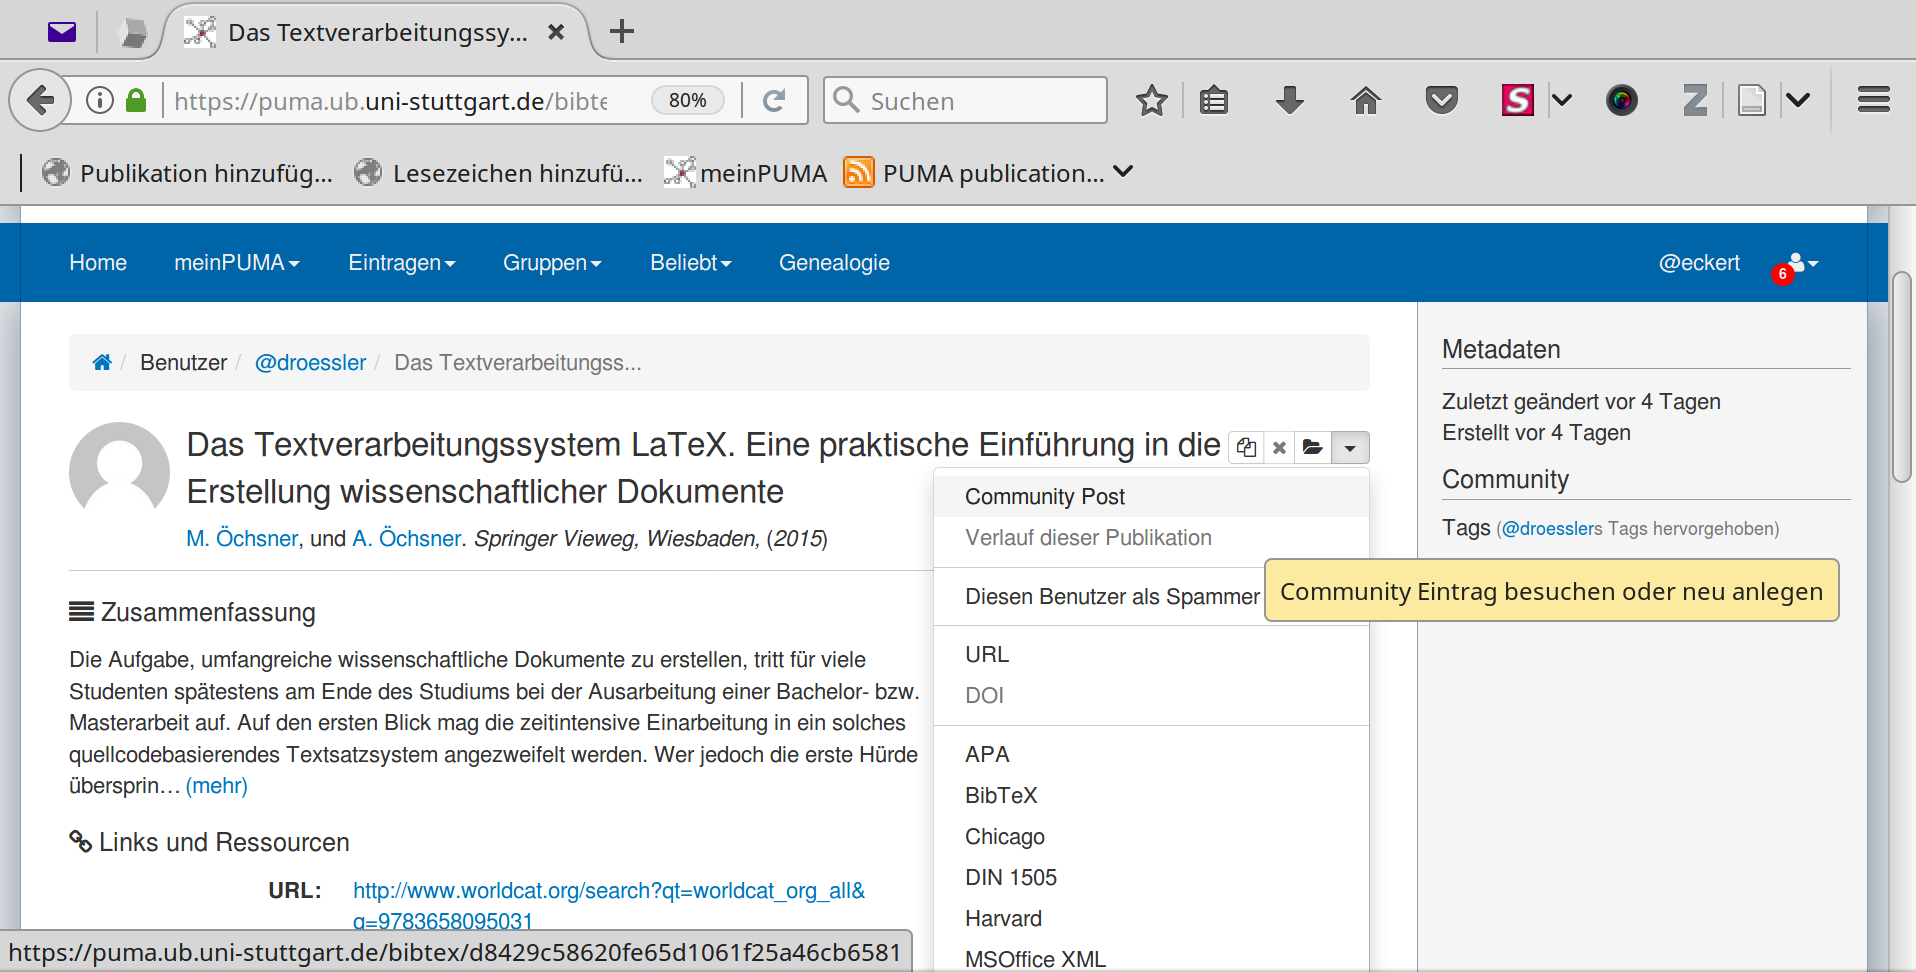
\includegraphics[width=11cm]{Bilder/Kapitel8/Community_post_anlegen}}
 \caption{Community Post anlegen}
 \label{fig:communityPostAnlegen}
\end{figure}
Der Community Post öffnet sich. Sie können nun Änderungen an der Publikation vornehmen, indem Sie oben links auf der Seite auf den Stift klicken, oder weiter unten auf der Community-Seite die Publikation bewerten. Die Änderungen werden in einer Übersicht - der Versionsgeschichte\index{Versionierung} - dargestellt. Zu dieser gelangen Sie oben links, durch einen Klick auf das Verzeichnissymbol.\newline
Durch die Erstellung eines Community Post können Nutzer jederzeit auf die Versionsgeschichte des Eintrages zugreifen und sehen, was und wann von wem geändert wurde. So erleichtert er die Zusammenarbeit und ermöglicht einen umfassenden Überblick. 

Im Bereich \textit{Tags} werden die Tags des Gemeinschaftseintrags angezeigt. Durch einen Klick auf einen Tag werden einem alle Publikationen mit diesem Tag angezeigt.

Unter dem Bereich \textit{Nutzer} werden alle Nutzer angezeigt, die diese Publikation in Ihrer Sammlung eingetragen haben.
\begin{figure}[h!]
 \centering
 \fbox{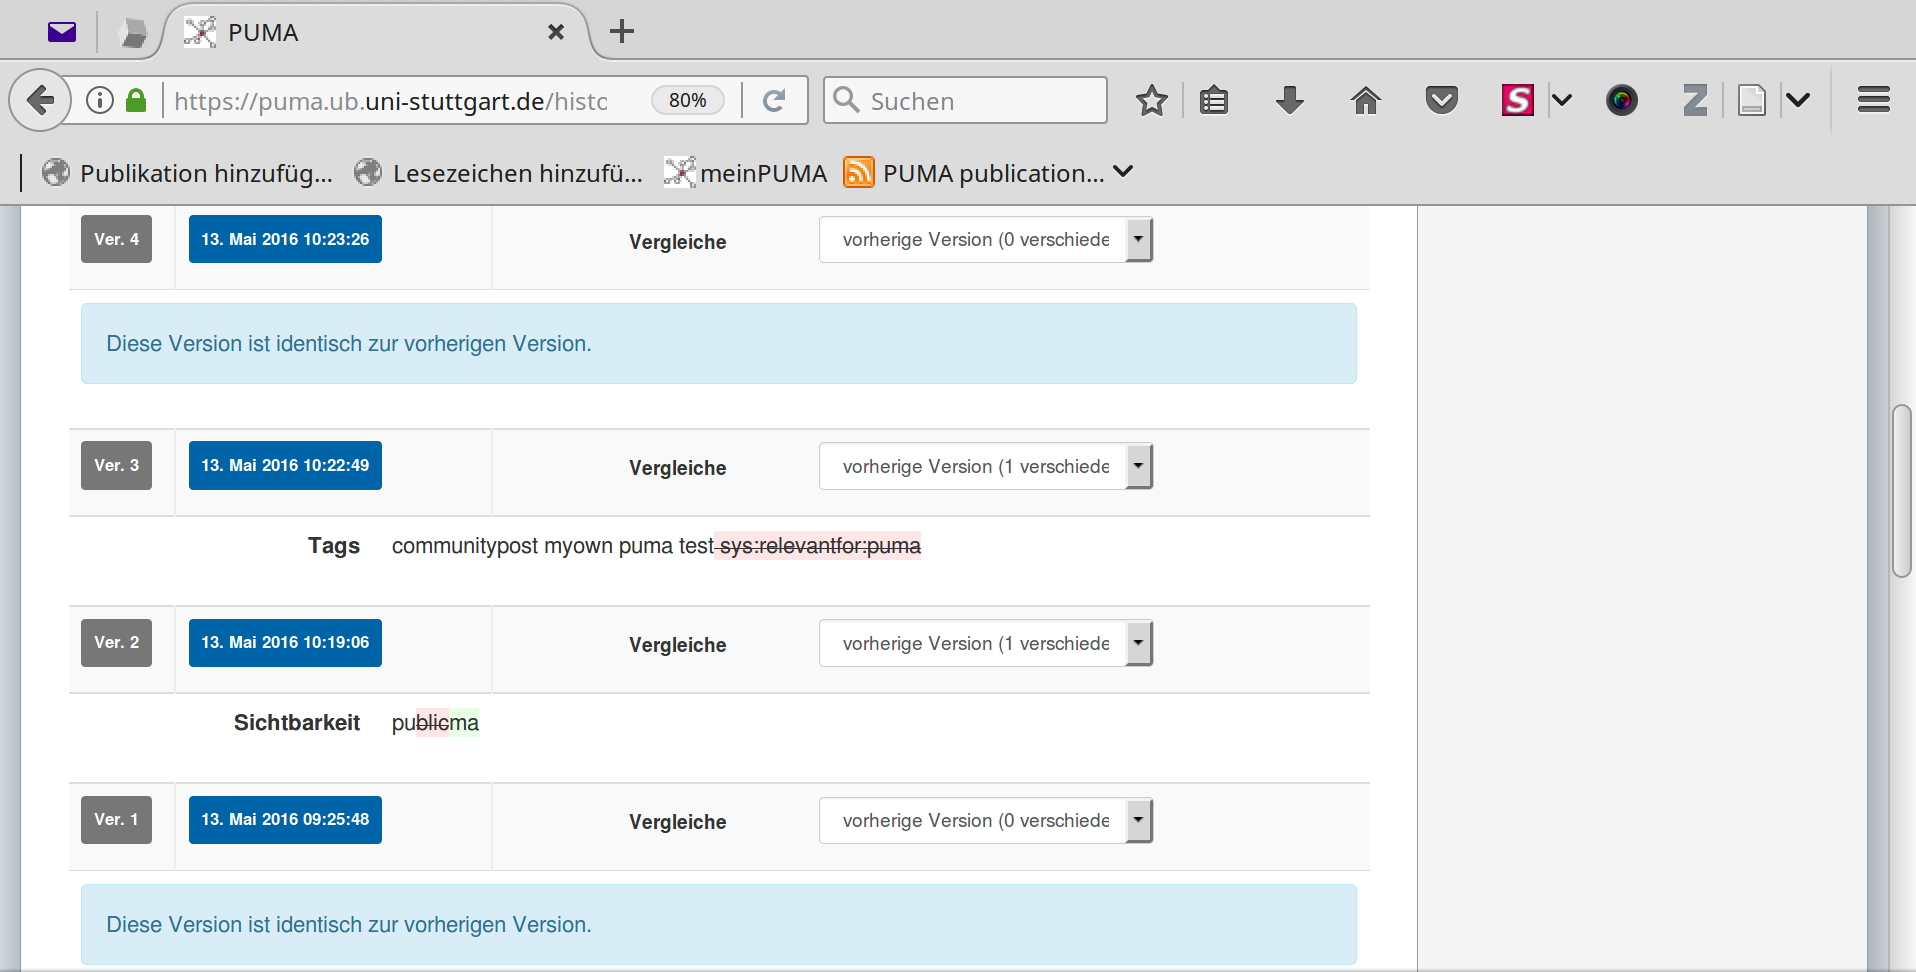
\includegraphics[width=11cm]{Bilder/Kapitel8/Community_post_Versionsgeschichte}}
 \caption{Versionierung}
 \label{fig:versionierung}
\end{figure}
\section{Nutzern folgen}
\label{sec:nutzernFolgen}
Wie in sozialen Netzwerken bietet PUMA seinen Nutzern die Möglichkeit, anderen Nutzern zu folgen. 

Um einem Nutzer zu folgen, gehen Sie auf dessen Benutzerseite (\autoref{subsec:freundHinzu}). Klicken Sie rechts oben, unterhalb des Benutzerprofilbildes, auf das Feld \enquote{folgen}. Ab sofort sind Sie ein Follower des Nutzers. Sie können jedem Nutzer folgen, egal ob befreundet oder nicht. \newline \newline
Um eine Überblick über die Einträge der verfolgten Person zu erhalten, klicken Sie im Reiter \enquote{meinPUMA} (\autoref{subsec:meinPuma}) auf den Unterpunkt \enquote{verfolgte Einträge}. Es erscheint eine Übersichtsseite mit allen Einträgen der Nutzer, denen Sie folgen. 




%Überarbeiten:neue version anders

\section{Kommentare, Rezensionen und Bewertungen}
\label{sec:kommentare}
PUMA verfügt über die Möglichkeit, Publikationen und Lesezeichen zu bewerten\index{Bewerten} und Rezensionen\index{Rezensionen} zu verfassen. Man kann mit anderen Nutzern über Publikationen/~Lesezeichen diskutieren und seine eigene Meinung zu einer Publikation/~einem Lesezeichen durch die Vergabe von Sternen verdeutlichen.
\newline
\newline
Publikationen/Lesezeichen bewerten:
\begin{enumerate}
    \item Klicken Sie auf die Stern-Leiste (siehe \autoref{fig:sternenleiste}) unterhalb des Lesezeichens oder der Publikation, die Sie bewerten möchten.
\begin{figure}[h!]
 \centering
 \fbox{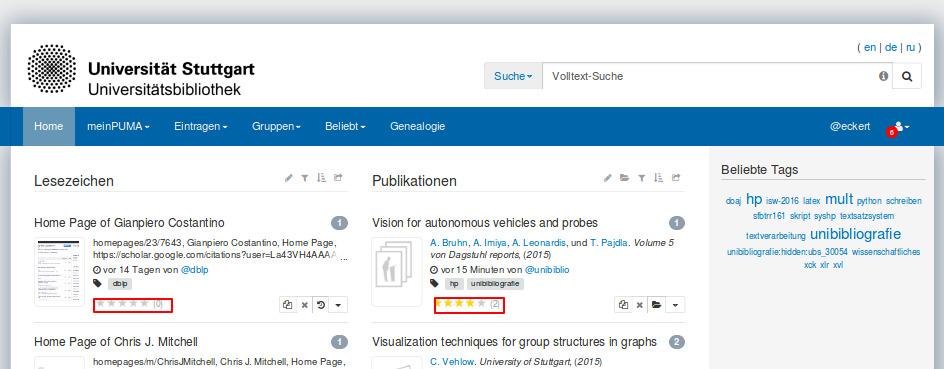
\includegraphics[width=11cm]{Bilder/Kapitel8/Die_Sternenleiste}}
 \caption{Die Stern-Leiste}
 \label{fig:sternenleiste}
\end{figure}  
    \item Es öffnet sich die Gemeinschaftsseite des Eintrages. Neben den Bereichen \textit{Tags} und \textit{Zitieren Sie diese Publikation} finden Sie hier auch den Bereich \textit{Kommentare und Rezensionen}. \autoref{fig:publikationBewerten} zeigt die Elemente des Bereichs:
\begin{figure}[h!]
 \centering
 \fbox{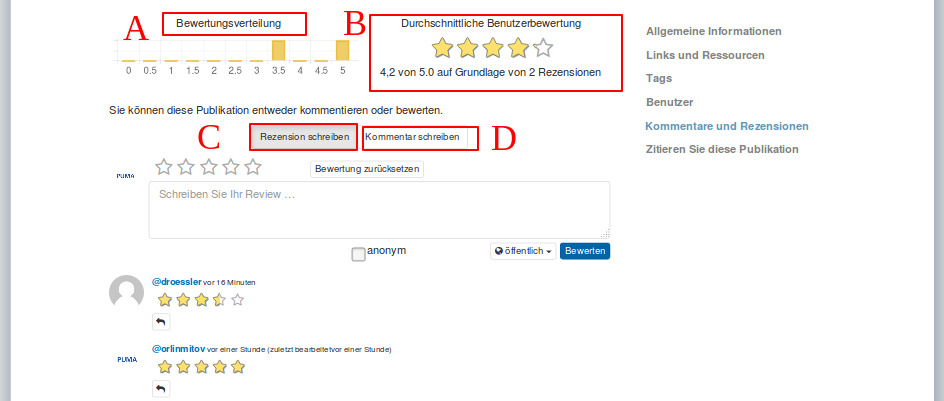
\includegraphics[width=11cm]{Bilder/Kapitel8/Publikation_bewerten}}
 \caption{Publikation bewerten}
 \label{fig:publikationBewerten}
\end{figure}
    \begin{description} 
        \item [Bewertungsverteilung (A):] Das Balkendiagramm stellt dar, welche Bewertungen wie oft vergeben wurden.  %In diesem Fall ... Beispiel an Hand eines Bildes
        \item [Durchschnittliche Bewertung (B):] In der Stern-Leiste wird der Mittelwert der Bewertungen angezeigt.
        \item [Rezension schreiben (C):] \hfill \\
				Durch einen Klick auf den Button "Rezension schreiben" öffnet sich ein Textfeld, das Ihnen die Möglichkeit bietet, ein Review zu verfassen. Oberhalb des Textfeldes können Sie den Beitrag mit null bis fünf Sternen bewerten. Je höher die Anzahl der Sterne, umso besser ist die Bewertung. Unterhalb des Textfeldes können Sie die Sichtbarkeit Ihrer Bewertung festlegen und so entscheiden, wer sie sehen darf. Es gibt folgende Möglichkeiten:
        \begin{enumerate}
            \item öffentlich: Jeder Nutzer kann Ihre Rezension sehen.
            \item privat: Nur Sie können Ihre Rezension sehen.
            \item Freunde: Sie können einzelne Freunde festlegen, die Ihre Rezension sehen sollen.
            \item Gruppen: Es werden Ihnen alle Gruppen angezeigt, in denen Sie Mitglied sind. Wählen Sie aus, welche Gruppe die Rezension sehen soll.
            \item anonym: Ihr Kommentar wird ohne Ihren Benutzernamen veröffentlicht. Die Bewertung ist für alle Nutzer sichtbar.
        \end{enumerate}
       	Klicken Sie abschließend auf \enquote{Bewerten}, um die Rezension abzuschließen und sie sichtbar zu machen.
        \item [Kommentar schreiben (D):] \hfill \\
				In diesem Textfeld können Sie einen Kommentar verfassen. Ein Kommentar hat die gleichen Möglichkeiten der Sichtbarkeit wie eine Rezension.
\newline Es kann beliebig oft auf Kommentare/~Bewertungen reagiert und geantwortet werden. Neben jedem Kommentar befindet sich ein Button mit einem kleinen schwarzen Pfeil, über den Sie Rezensionen direkt kommentieren können. 
    \end{description}
\end{enumerate}